% This document will contain some of the preliminary research and findings that I've been working on.
%
%
%
\documentclass{report}
\usepackage{amsmath}
\usepackage{graphicx}
\usepackage{setspace}

\graphicspath{Images and Figures}

\title{Maritime Cybersecurity}
\author{William Smith}

\begin{document}
\maketitle
\doublespacing

\begin{abstract}
Systems on board ships have become increasingly interconnected, which raises questions concerning the security of critical systems. Due to the intrinsic nature of the industry, maritime systems and standards have had little motivation to change in favour of more advanced equipment, and much of the industry still relies on decades old software and communication standards. A closer look at how these systems are connected and how they communicate will lead to further discussion on the integrity of these practices. This paper will analyze shipboard networks from a top-down approach, beginning with network architecture analysis and the different approaches taken depending on the purpose of the network, and eventually summarizing the communication protocols used in serial networks. Finally, some suggestions are made on ways to design and implement a test bed that can simulate the systems on board a ship, which could prove useful for future research and testing. 
\end{abstract}

\tableofcontents

\chapter{Introduction}

With the introduction of technologies such as Automated Information Systems (AIS) that have become mandatory on board certain ships, shipboard systems have become increasingly inter-connected. In order to properly analyze the security implications of shipboard systems, it is crucial to have an in depth understanding of ship data network standards and in what ways these technologies will proceed in the future. This report will include a comprehensive analysis on the different communication standards that are used to connect devices within an on-board ship network, as well as providing some context to the architecture of shipboard networks. Once questions concerning how ship networks are typically configured, as well as the inner working of the protocols used in these networks are answered, functional models can begin to be made and testing can begin. Testing would provide a platform to discover vulnerabilities, and recommendations can be made about how to safely integrate marine systems in the future. 

\chapter{Shipboard Network Architecture}

Ships are made of several interconnected systems that are constantly communicating with each other. Ships are often likened to small autonomous villages with systems for power distribution, propulsion, navigation, life support, cargo monitoring, and control systems[5]. Manufacturers control how these systems interact with each other, only adhering to certain lower level communications standards. It is up to manufacturers of these systems to determine how they want to implement an integrated system. There does however happen to be guidelines set by organizations that look to govern the landscape of shipboard networks to ensure safety. The International Association of Classification Societies (IACS) has recent publications of their recommended network architecture guidelines which covers design, installation, and testing of proposed networks. The IACS claims that more than 90\% of the world's cargo carrying tonnage is covered by the classification design, construction, and through-life compliance rules and standards set by the its twelve members. This is supported by the fact that their network architecture overview closely resembles the network solutions offered by notable marine technology manufacturers. Such shipboard networks are generally comprised of distributed control systems (DCS) and its associated devices, programmable logic controllers (PLC) and its associated devices, routers and switches, human machine interface units, and computers. This validates many of the automated control network solutions offered by companies such as Samsung, Mitsubishi, Noris, and Wartsilla.  Networks on board are split into two categories based on their functionality: the ship administrative network that consists of computers that perform administrative tasks such as communication with shore offices, and the ship control network that consists of several individual and integrated systems to control specific functions of the ship. These networks are often segregated and segmented into various zones by risk level. This is done either by using physically different networks, or by using logically different networks by using a virtual private network (VPN). Should devices need access to a network outside its zone, it should be controlled at the perimeter using protection devices such as proxies, gateways, firewalls, and encrypted tunnels [10,16]. 

\section{Ship Control Network}
The following sections show the ship control network split into two sections: the navigation bridge and the engine control automation network. Figure 2.1 shows a high level depiction how the networks on each section is generally configured. This diagram is based on the a number of notable system manufacturers' control network solutions. There are some important distinctions between the two networks, most notably the communication protocols used for device communication. Based on available sources, there few manufacturers that show a distinct link between the two networks, but it is unclear how they interact with each other .  

\begin{figure}[h]
    \centering
    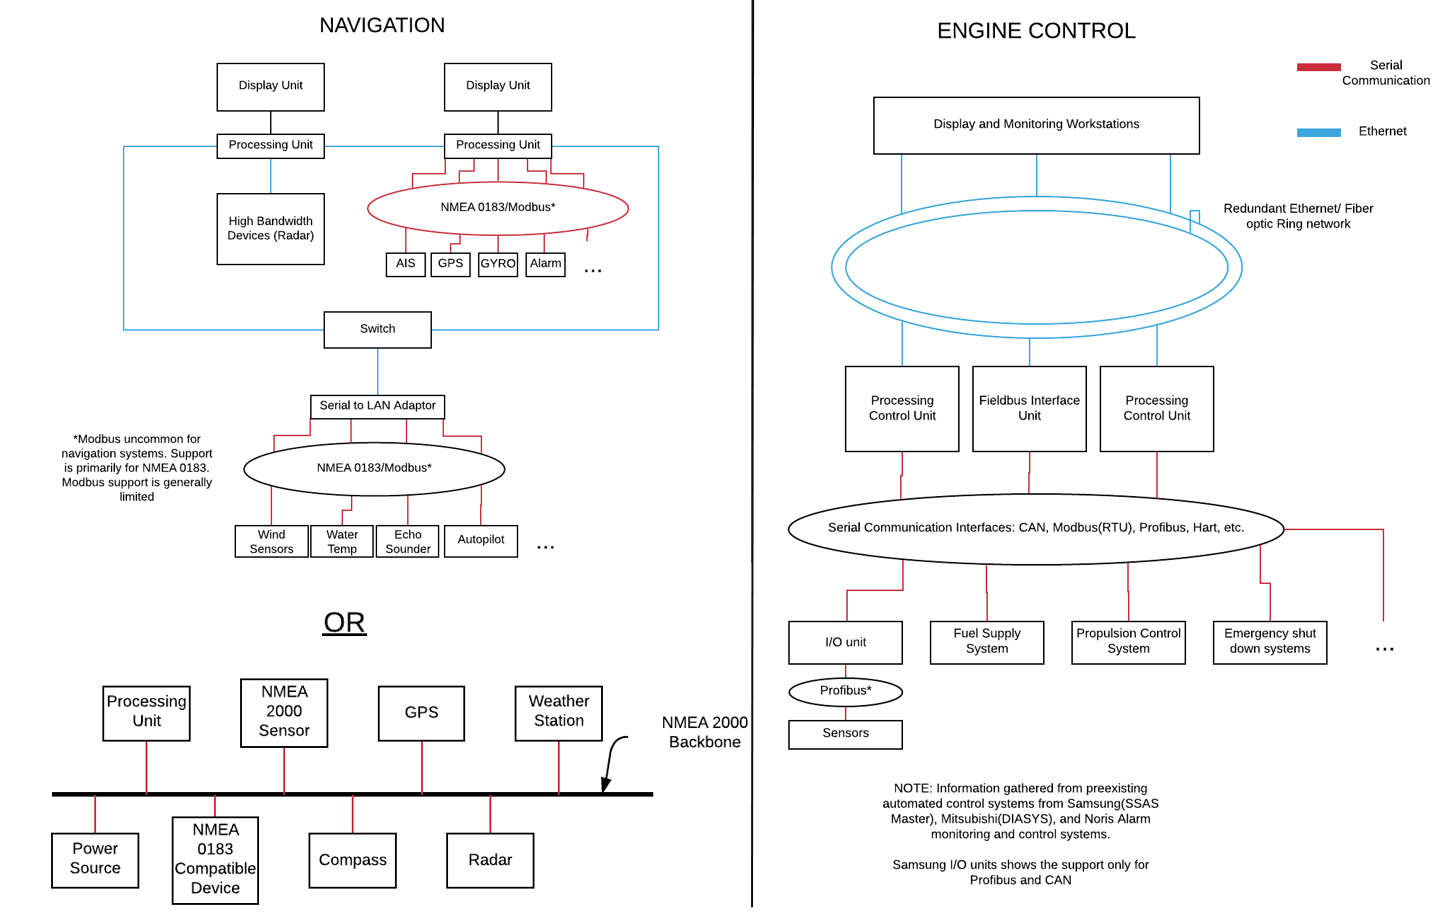
\includegraphics[width=12cm]{Images and Figures/High-Level Diagram.PNG}
    \caption{High level diagram of the ship control network }
    \label{fig:Navigation Bridge}
\end{figure}

\subsection{Bridge}
The ship's bridge is home to numerous highly interconnected systems that communicate with each other. The International Maritime Organisation defines an integrated bridge system as "a combination of systems which are interconnected in order to allow centralized access to sensor information or command/control from workstations, with the aim of increasing safe and efficient ship's management by suitably qualified personnel. Figure 2.1 shows the devices that are typically connected the bridge of a ship. ECDIS is one of the central points of connection for devices on the bridge and holds the details on how these devices communicate with other shipboard systems.
\vspace{5mm} %5mm vertical space
In Chapter V of The Safety of Life at Sea (SOLAS) convention published by the International Maritime Organization (IMO), Integrated Bridge Systems are to be arranged in such a way that if one sub-system fails, the rest of the network of systems are entirely unaffected [9]. This is accomplished through redundant connections that maintains the reliability of an entire network of systems should one device fail.

\begin{figure}[h]
    \centering
    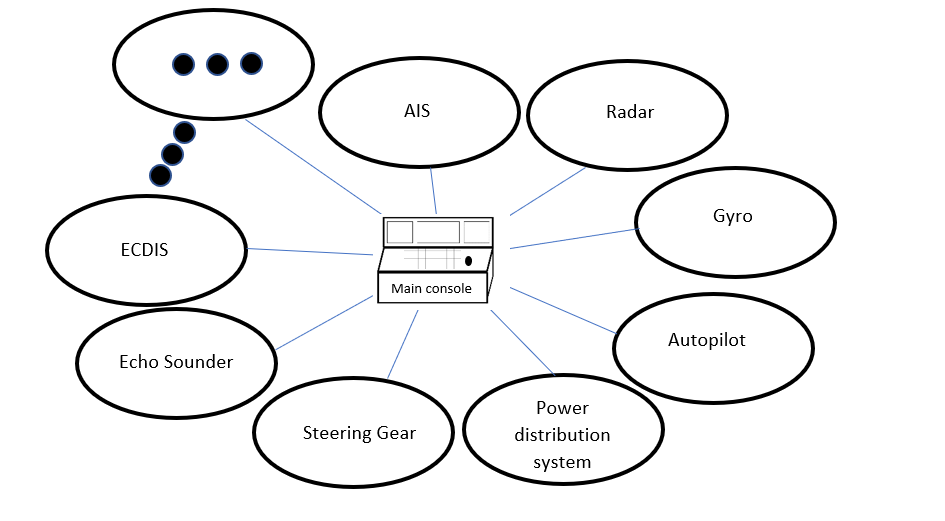
\includegraphics[width=12cm]{Images and Figures/Navigation Bridge.PNG}
    \caption{Interconnected devices making up the integrated bridge system. [5]}
    \label{fig:Navigation Bridge}
\end{figure}

\subsection{ECDIS and its Importance}

With on-board ECDIS workstations being one of the main convergent points in the network of systems and sensors on the bridge, ECDIS has been crucial part in understanding the network layouts on vessels using ECDIS solutions by common manufacturers. There are several different methods manufacturers are employing their networks, one of which is simply connecting the sensors directly to a main processing workstation, using the single talker, multiple listener IEC 61162-1/2 (NMEA 0183) standard, or other serial communications protocols like Modbus. Each of the ECDIS solutions offered by the Furuno, Transas, and the Maris ECDIS900 employ this method, where external devices and sensors such as AIS, GPS, Alarm Systems, and gyroscopes are connected directly to the processing unit, and additional sensors are connected to a serial to LAN adaptor that is either connected directly to the processing unit or to a switching hub as shown in Figure 2.3.These systems typically include support for numerous sensor adaptors, specifically to accommodate the need for redundancy.[6][7] 

\begin{figure}[h]
    \centering
    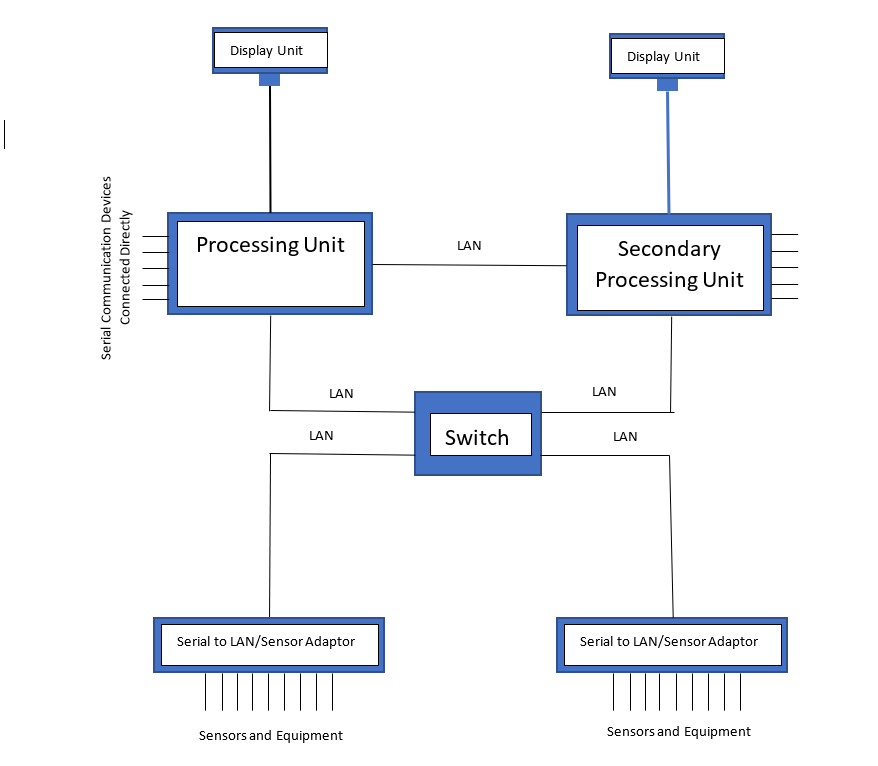
\includegraphics[width=12cm]{Images and Figures/ECDISsensorNetwork.PNG}
    \caption{ECDIS Sensor Network}
    \label{fig:network}
\end{figure}


\begin{figure}

\end{figure}

An alternate configuration exists in which other manufacturers opt to use the NMEA 2000 communication standard, which allows devices to be connected directly to the backbone cable and and communicate over a CAN bus network. This network configuration is less frequently implemented in large shipping vessels but is more widely used in smaller leisure vessels[5]. Simrad who offers ECDIS systems with smaller ships in mind, is a manufacturer whose solution follows this model. Simrad's wiring diagram is far simpler than that of the other previously mentioned manufacturers offering Ethernet and serial communication solution. Simrad's main workstation is connected to the backbone directly, along with any NMEA 2000 compatible sensors, the power supply, and terminator components on each end of the backbone[17]. Maretron, a company that offers marine vessel monitoring and control systems solutions, offers a free NMEA 2000 network building software that allows you to design entire ship networks on the backbone of the NMEA 2000 standard. The following is an example of a 50ft sailboat that is offered through the software as an example network. NMEA 2000 will be discussed in greater detail in the following chapter.
\begin{figure}[h]
    \centering
    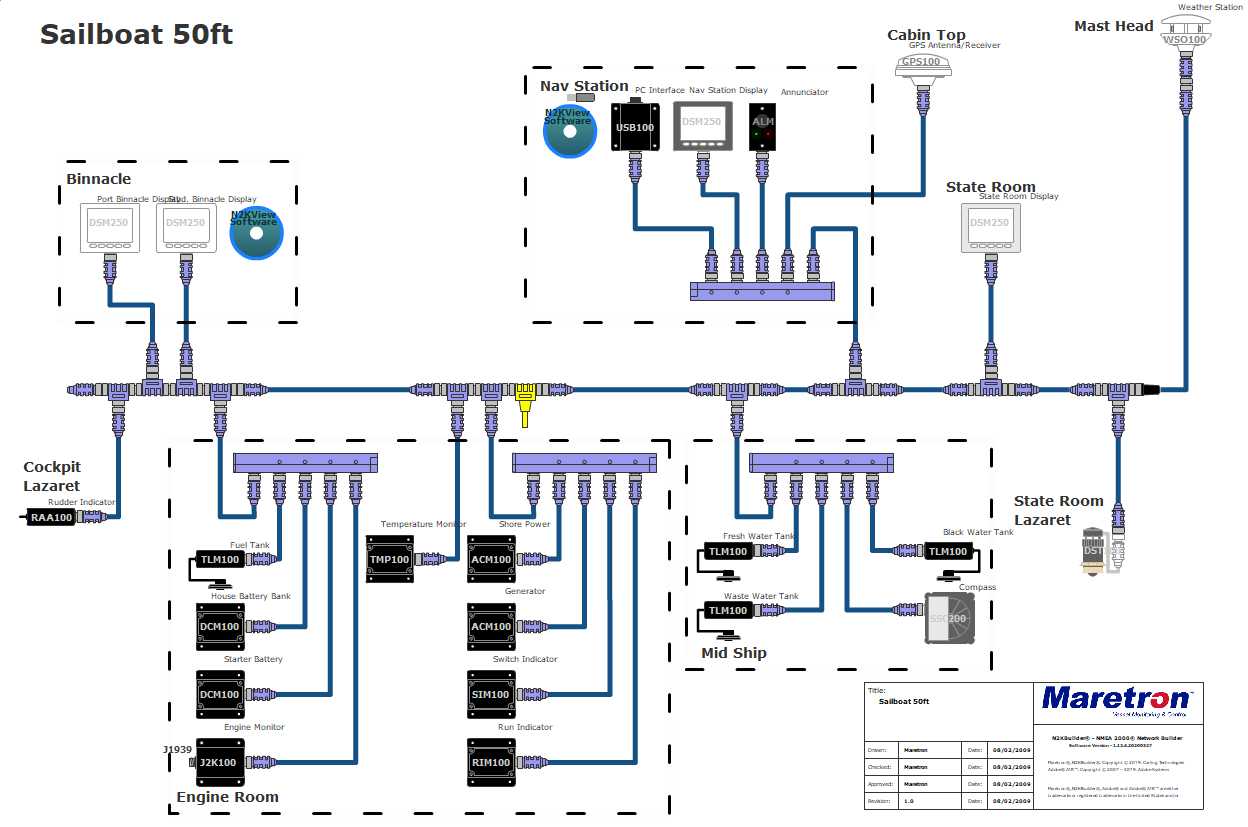
\includegraphics[width=12cm]{Images and Figures/NMEA2K.png}
    \caption{Example NMEA 2000 CAN Network on board 50ft sailboat [5]}
    \label{fig:NMEA CAN}
\end{figure}
 
\subsection{Engine Control Systems }

This portion of the ship controls many equally vital systems as the bridge does. Similar to the previous section, manufacturers have control over how they want systems to control the engine, boiler, cargo, turbine, power management, alarm systems, and other crucial functions are implemented. Such integrated systems are packaged by manufacturers as some form of "integrated automation systems". These systems will typically have all main displays and monitoring workstations connected to the main processing units and field bus interface units connect using a form of redundant Ethernet ring. The processing units are then connected to I/O units and other critical systems using standard field bus protocols such as Modbus, CAN, Profibus, and Hart as shown in figure 2.1. Some devices are specific to only one field bus protocol, but other devices may support numerous protocols. This is left up to the system manufacturers. 
\vspace{5mm} %5mm vertical space
An example of such a control system is employed by the company Maersk, A world-wide leader in overseas shipping and the owner of the largest commercial cargo vessel. Maersk vessels are powered by a diesel engine manufactured by Wärtsilä, and comes accompanied with the Wärtsilä Unified Control(UNIC) engine control system. This system is mounted locally on the engine in the form of a control panel and a display unit that shows critical operating data. The system has control over the engine's crucial operating functions such as its start/stop and  speed, as well as engine protection features such as alarms, shutdowns, and emergency stops. The controller uses the Modbus communication protocol to communicate with external systems either through Ethernet or serially.[3].  

\section{Ship Administrative Network}
There is a far greater emphasis on the ship control network from both governing agencies, as well as system integrators. This is likely due to the fact that should the charting workstation malfunction on board, there would likely be a greater immediate risk to the safety of shipboard operations than if a crew member had trouble accessing maintenance records or the passenger internet. 
\vspace{5mm} %5mm vertical space
The International Organization for Standardization (ISO) has published guidelines for installing communication networks on board ships, independent from navigational equipment networks and engine control networks. This publication stresses that there have not been comprehensive guidelines on such networks until now. This communication network will be connected to the navigational equipment network and the engine control network through the use of a gateway, but will not have control over their operation. There is little reference to this standard itself from external sources and no indication of its adoption rate or impact on the current market. On top of this, the specifications of this standard require purchase so they were not accessible at this time[15].

\section{Layered Shipboard Network Model and MiTS}

The Maritime Information Technology Standard (MiTS) was first published by a Norwegian research team during 1991 and 1993. This standard looked to comply with a trend that saw all vital systems beginning to interface with one another to form an integrated system. Their main goal through the MiTS integrated control and open systems standard was to make better systems that are both more secure, and make the lives of operators easier. Uptake of MiTS was slow, partially due to the lack of redundancy support which is crucial for ships containing critical systems. Despite this, MiTS had a very notable impact on the industry and allowed for the creation of other protocols, most notably Light-Weight Ethernet (IEC 61162-450) that will be discussed in greater depth in the following chapter. The design philosophy of MiTS researchers during this time was to choose standards that have already been established like TCP/IP, and to select low level protocols for communication protocols in lieu of high level ones. Mits introduced a layered network model which has been updated with more relevant layers to meet today's standards and it continues to be a commonly used reference model today[5].


\subsection{Network layout}

Ships are made up of several complex interconnected systems, with each part complying with multiple industry standards depending on the manufacturer. Without a one size fits all solution for how layered ship networks are constructed, a general model can be used and a number of manufacturers can be compared for differences and similarities in their network solutions. The typical reference model a ship network architecture is one in which there are multiple layers, each of them connected to each other either through applications, generic firewalls, or gateway components. Figure 2.5 shows the modernized version of the model which includes a general ship layer, as well as an off ship layer, both of which didn't exist at the time layered networks model's conception[5].
\begin{figure}[h]
    \centering
    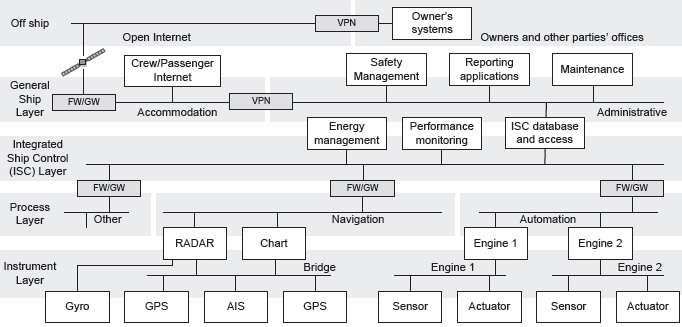
\includegraphics[width=12cm]{Images and Figures/isc-arch.jpg}
    \caption{Schematic Ship network Architecture[5]}
    \label{fig:network}
\end{figure}


\subsection{Instrument Layer}
The first of the five layers is the instrument layer, which is made up of several more simple devices and sensors that are connected to higher level components that use them. The lower level devices and sensors are typically connected to higher level systems using an industrial field bus protocol such as NMEA 0183, NMEA 2000, Modbus, Profibus, or others.

\subsection{Process Layer}
The process layer ensures that all of the ship specific functionalities are integrated in a single process segment such as navigation or engine control.
\subsection{Integrated Ship Control Layer}
The integrated ship control layer is the top layer in the trusted part of the system. This layer makes the sure the different process segments are interconnected as needed, and bridges over to the administrative networks when required. As shown in Figure 2.5, each process segment is connected to the integrated ship control layer through the use of a gateway or firewall. This is crucial as one problem in the integrated ship control layer can propagate down many layers, and affect the critical systems on board.
\subsection{General Ship Layer}
The general ship layer includes less critical ship functions such as crew and passenger internet and the administrative functions of the ship. 
\subsection{Off-Ship Layer}
The final layer consists of networks on shore that usually connect to the ship via satellite. This will often include the owner or the operator's systems that are connected through secure data links by using a VPN[5]. 


\chapter{Currently Used Communication Standards}
\section{NMEA 0183}
The National Marine Electronics Association (NMEA) is a US based association that looks to create uniformity of electrical standards among manufacturers. This has been accomplished through the NMEA 0183 standard which has been widely accepted by manufacturers worldwide. NMEA 0183 has been available since 1983 and the newest version published in November 2018 continues to be widely used today. This standard uses the RS-422 electrical standard (most NMEA 0183 compatible devices also capable of driving a single RS-232 port) and uses an ASCII serial communications protocol that defines how data is transmitted by a single talker as sentences over a serial data bus for one or more listeners. NMEA is relatively slow, supporting a bandwidth of only 4800 bps and without the support for multiple talkers, it is not capable of creating networks. In leisure vessels, NMEA 0183 continues to be slowly phased out as the newer NMEA 2000 standard is replacing it, however, it continues to remain the go-to in commercial shipping applications.
[wiki and NMEA.org, ]  

\subsection{NMEA 0183 Technical Specifications}

As previously mentioned, NMEA 0183 sentences are sent over the RS-422 electrical standard. RS-422 uses a multi-drop bus, allowing for a single driver and multiple receivers. While limited to a unidirectional data transmission, a line length of up to 1200 m is supported, it is suitable for noisy environments, and is a well established standard[13].
\vspace{5mm} %5mm vertical space
NMEA 0183 data is sent in the form of plain ASCII text with the following format:  

\begin{center}
    \$yyXXX,............*xx$<$0D$><$0A$>$
\end{center}

The sentence will always begin with either a '\$' or '!', with each subsequent part of the sentence separated by commas. The two character length "yy" code indicates the type of device that is transmitting data. In the case of a GPS or a depth sounder, the "yy" code will read as "GP" and "SD" respectively. The following three digit "XXX" code indicates the data type of the sentence. A data type of Global Positioning Fix Data will read as "GGA". After the previous two codes, a comma will separate what is the contents of the data which will differ depending on the data type and the readings from the sensors. The final "xx" characters are an optional two digit checksum that is generally included to safeguard the data in the sentence. The checksum is calculated by taking the 8-bit exclusive-OR of all characters including all ',' and excluding the '\$','!', and '*' delimiters. The sentence will always terminate with a carriage return and a line feed.
\vspace{5mm} %5mm vertical space
As an example, a temperature sensor is on board a ship and transmitting NMEA 0183 sentences to the navigation system describing the mean temperature of water in degrees Celsius. The format of this message will be in the form:  
\begin{center}
    \$xxMTW,DATA\_TEMPERATURE\_C,C*hh$<$0D$><$0A$>$
\end{center}
The message shows that the data type will be of type Mean Temperature of Water. A complete sentence that a sensor may transmit would read as the following:  
\begin{center}
    \$YXMTW,17.75,C*5D$<$0D$><$0A$>$
\end{center}

Where the device code is indicating that the transmitting device is a transducer and the temperature reading is 17.75 degrees Celsius[12].

\section{NMEA 2000}
NMEA 2000 is the newer, more sophisticated standard that is the successor to the NMEA 0183 standard. The purpose of NMEA 2000 is to create a single wire feed that acts as a backbone, with external devices and sensors connecting via a "Tee" connector piece, and a terminator connector on each end of the backbone. Another aspect in which NMEA differs is in how devices communicate with each other using this standard. NMEA 2000 compatible devices are connected using CAN (Controller Area Network) technology, and allows for the transmission and reception of data from multiple devices simultaneously. This makes it possible to implement integrated navigation and control systems solutions on board vessels of varying sizes. NMEA 2000 transmits data at a significantly higher rate than NMEA 0183 at speeds up to 250 kbps. It is common to find devices that process high volumes of information such as radar, electronic charts, and weather overlay information offer both Ethernet and NMEA 2000 connectivity. Where Ethernet is at a disadvantage is that there is no marine standard, making it not guaranteed that devices from different manufacturers are capable of communicating with each other. Ethernet also cannot prioritize the transmission of important information the same way NMEA 2000 can. Should multiple devices choose to communicate at the same time and a bus conflict occurs, with CAN, the device with the highest priority will go ahead with the transmission, and the lower priority device will try again later, where as with Ethernet the devices causing the collision will simply both stop transmitting and will try again later. This makes CAN a better suited solution for critical applications that require immediate response such as steering.
[7]   

\section{NMEA 2000 Technical Specifications}

NMEA 2000 data messages differ greatly from its predecessor. Rather than transmitting ASCII text sentences, NMEA 2000 transmits messages as a series of data frames. Each frame is made up of error checking and data delivery confirmation bits, a 0 to 8-byte data field, and a 29 bit identifier that sets message priority, as well as identifies the message, its source, and its destination. The actual data contents of an NMEA 2000 frame typically makes up less than half of the transmitted bits. This lends itself well to most maritime equipment as they typically send fairly short data messages. There is extensive error checking that occurs when a frame is transmitted. 15 bits of the frame are entirely devoted to a cyclic redundancy check for error detection. Five different error checks are conducted per frame, and up to six errors can be recognized in a single frame. Each message sent by a talker is ether excepted by all other nodes, or none. 



\section{IEC 61162}
The International Electrotechnical Commission is the world leader in preparing and publishing international standards for a wide variety of electrical and electronic technologies. The IEC 61162 standards are a set of electrical communication standards strictly relating to "Digital interfaces for navigational equipment withing a ship". Each part of the IEC 61162 set of standards deal with the transport of NMEA sentences. a IEC 61162 includes NMEA 0183 in the form of IEC 61162-1, NMEA 2000 in the form of IEC 61162-3, and NMEA 0183 messages transported over IPv4 via Ethernet in the form of 61162-450, also known as Light Weight Ethernet (LWE) for its low protocol complexity. LWE was developed with the intention of allowing efficient interfacing of equipment between manufacturers, as nearly all manufacturers simply have their own integrated bridge network solutions, which are typically based on Ethernet. LWE is intended to be used as an instrument or process layer network.
\vspace{5mm} %5mm vertical space
The last of the two standards defined by IEC 61162 are incremental upgrades in the form of a faster rate of data transmission for single talker and multiple listeners as IEC 61162-2, and a more secure add on to LWE as IEC 61162-460. There are very few implementations of IEC 61161-460 as it is a relatively new standard. More information on each of these standards are available through IEC but require purchase[5].

%\section{talk about field bus a little bit...}
%modbus, profibus, and others...

\chapter{Creating a Model}

buying the NMEA 0183 standard is a little expensive, however much of it has been reverse engineered and is available for free online. This could be used in simple proof of concept tests. (more here)

\section{Bridge Simulation Design}

The bridge is often made up of interconnected typical workstation PCs running some form of windows, with some proprietary software installed to serve its purpose. ECDIS systems for instance, operate in much the same manner. There were two main considerations when approaching the problem of creating a simulated bridge system. The first was to look through the hardware specifications of popular ECDIS systems and in theory, it would be possible to construct a workstation that matches the hardware specifications down to the motherboard, CPU, RAM modules, etc. The ECDIS installation manual for the Transas NAVI-SAILOR 4000/4100 provides such a detailed list of hardware specifications for their system. This also includes a Peripheral Component Interconnect Express (PCIe) expansion card that adds four serial ports to the system, which is noteworthy as it would be compatible with other systems[6]. This however does not address the issue of obtaining the proprietary software needed to complete the system, and the feasibility of this solution may also be in question a potential issue in gathering the required legacy hardware. If the exact hardware specifications are not needed, you could simply insert the PCIe card into any modern PC, provided that there is an available expansion slot on the motherboard. This would be enough for a small subsystem of devices for testing.
\vspace{5mm} %5mm vertical space
A different approach could be taken in which the ECDIS system is simulated by other means. One common DIY electronic chart solution for smaller vessels is one in which a Raspberry pi (or any other small single board computer) with some open source software is used to simulate an ECDIS system. This type of solution would not qualify as ECDIS as such a system is not certified under the IMO, but would functionally serve the same purpose. There are numerous open-source software resources such as OpenPlotter, which is an sailing platform developed specifically for ARM based computers. OpenCPN is another free piece of software that serves as the main electronic charting system. OpenCPN and OpenPlotter are both NMEA compatible, however some extra hardware is required in order for NMEA devices to interface with the Raspberry pi. By default, there is no support for the RS-232/422/485 electrical standards, so a USB converter or the RS-422/485 HAT for Raspberry Pi is required[NMEA raspberry pi]. While many of the known security vulnerabilities found in ECDIS systems are a result of underlying operating system vulnerabilities that are not relevant to this particular solution, there are still questions concerning the integrity of the electronic charting system should one or multiple devices fail.[11]
\vspace{5mm} %5mm vertical space
After employing an ECDIS system of choice to simulate the bridge of the ship, there are a number of peripheral devices needed to fully complete the test bed. The most obvious approach to accomplishing this would be to simply obtain an NMEA device such as a GPS or an auto pilot have those devices communicate with our electronic charting workstation. This would be valuable in terms of transmitting real NMEA sentences. A software alternative to this can be accomplished as well through the use of NMEA sentence simulators which will turn a computer into an NMEA device with the help of a USB to RS-422/485 adaptor. This way the type of device to be simulated and the sentences transmitted would be up to the user. Such a simulator is available through the company NMEAsoft, a company that specializes in marine navigation equipment simulation. NMEAsoft also has software to simulate GPS data, as well as a NMEA monitoring program that will monitor NMEA messages. This software is costly though, and there are free alternative simulators and monitors available, one of which comes in the form of as Chrome browser extension. 
\vspace{5mm} %5mm vertical space
Finally, PyNMEA is an open-source library written in Python that allows for parsing NMEA 0183 sentences, as well as generating sentences from data. This could be a monitoring solution itself, and perhaps a device could be programmed to monitor and log NMEA data. As previously pointed out, NMEA sentences appear in plain text, and this makes NMEA devices susceptible to middle person attacks. A device could be created using PyNMEA to intercept messages and modify them however the user would like. This would help to understand the extent of damage that could be caused by such an attack. Other attack strategies could be employed as well such as GPS spoofing and jamming signals in order to observe how the system responds. Deploying such a device should be relatively simple, since the RS-422 electrical standard allows for a multi-drop interconnect comprising of a single driver and multiple receivers, hence the single talker multiple listener description of NMEA 0183, it should be as simple as setting up the device as another receiver/listener, and log the data from there. 
\vspace{5mm} %5mm vertical space
Another consideration may be a vessel that uses the NMEA 2000 protocol. Although less frequently implemented, it has had market penetration in smaller ships. The Raspberry Pi running OpenPlotter has full support for NMEA 2000, however there are fewer monitoring and simulating solutions. Would a wire tap on the backbone of the bus work to monitor all the data?

\section{Engine Control Network Design and Challenges}

In terms of a hardware solution to accurately portray the workings of an engine control network would require some costly proprietary equipment. Data monitoring solutions can still be developed and tested. The most common field bus protocols utilise the same RS-485 multi-point standard. This should make for fairly straight forward monitoring of any of the protocols. Some work has already been completed a systematic approach to building a passive monitoring system for Modbus networks[14]. Modbus would likely be an appropriate protocol to focus on for an engine control system as it is widely used and it is an  openly published standard. A small Modbus network of devices simulating the functions of a ship may be sufficient for the purposes of this project. This could be accomplished very simply by using RS-422/485 adaptors along with a some simple inexpensive microcontrollers. There exists resources that explain how to configure Arduino to operate using Modbus. In the case of using an Arduino, a TTL to RS-485 converter is needed.



\section{SATCOM Interception}
There has been some recent research conducted by an Oxford University-based researcher James Pavur, who has found a way to intercept critical shipboard satellite data by using widely available and inexpensive hardware tools to scan for internet service and interpret the data. Pavur bought a flat panel television satellite dish and TBS-6983/6903 PCIe card to process the signals. He then used a tool called EBSpro to find satellite internet traffic. Once he finds a satellite, he uses TBS Recorder to record traffic, and uses other software tools to extract meaningful data from the broadcasts. Due to satellites being positioned far away, there can be several hundred milliseconds of latency, and encrypting the broadcasted data can even further hinder performance. For this reason, Pavur found that much of the traffic he intercepted appeared in plain text with no encryption. Pavur investigated 12 ships ranging from small fishing vessels to several vessels carrying greater than 100,000 tonnes of cargo and logged their traffic. He found instances of publicly routable FTP fileshares containing chart updates occurring with the password to the server being transmitted in plain text over satellite, as well as emails containing chart updates that could leave the crew susceptible to targeted email phishing attacks. SATCOM security has not been identified as a major threat to maritime cybersecurity by many researchers, so more work such as this needs to be done in order to stop a potentially new avenue for attackers[18].



\chapter {Recommendations and Conclusion}

“Maritime Cyber Security Analysis – How to Reduce Threats?” names the following five areas susceptible to cyber attacks: Navigation Bridge, Power Management Systems, Engine Room, Cargo Handling Equipment, and Administrative and Communicational Systems[1]. This is a very high level depiction of the state of maritime cybersecurity, and it may hide some of the finer details that are at risk of exploitation. Rather than look to identify the bigger picture threats that have been previously identified, a more focused approach was taken to better understand the inner workings of systems on board and how they interact, which will hopefully lead to discoveries of underlying issues in the industry.
\vspace{5mm} %5mm vertical space
There are many challenges with choosing ship data network methodologies. Ships are complex entities with many interconnected systems working together and relying on each other. It is often easier to go with a proven existing standard or piece of software than to create one from scratch. This is particularly important as ships generally have a lifespan of anywhere from 25 to 35 years. While employing trusted standards is not inherently bad, the maritime industry continues to use decades old technology that has fallen behind much of the technological world. With critical workstations running old operating systems with known critical security vulnerabilities and electronic charting systems being updated with charts received over email, there are clear areas for improvement in the industry. Some manufacturers have led the way in this area by using the latest standards and by making the point to stop unsafe practices, but there continues to be widespread use of outdated design strategies. Old industry habits aside, one thing is clear; there needs to be an increase in standardized security support, particularly in the form of remote monitoring to know exactly the moment something goes wrong, as well as improved maintenance capacity to fix issues immediately. 
\chapter{References}

Mraković, I., \& Vojinović, R. (2019). Maritime cyber security analysis – How to reduce threats? Transactions on Maritime Science, 8(1), 132–139. https://doi.org/10.7225/toms.v08.n01.013 [1]

Balduzzi, M., Pasta, A., \& Wilhoit, K. (2014). A security evaluation of AIS automated identification system. ACM International Conference Proceeding Series, 2014-Decem(December), 436–445. https://doi.org/10.1145/2664243.2664257 [2]

Wärtsilä. (2016). Wärtsilä UNIC engine control system for diesel engines. 2. [3]

Dyryavyy, Y. (2015). Preparing for Cyber Battleships – Electronic Chart Display and Information System Security.[4]

Rødseth, Ø. J. (2006). Design challenges and decisions for a new ship data network. 450.[5]

Transas. (2009). NAVI-SAILOR 4000/4100 ECDIS Installation Guide.[6]

Krile, S., Kezić, D., \& Dimc, F. (2013). NMEA communication standard for shipboard data architecture | NMEA komunikacijski standard za arhitekturu podataka na brodu. Nase More, 60(3–4), 68–82.[7]

Furuno (2018). Installation Manual. - furuno ecdis 3200 installation manual[8]

International Maritime Organization. (2002). Safety of Life at Sea - Safety of Navigation Chapter V. SOLAS Convention, 29.[9]

IACS. (2018). No. 156 Network Architecture Contents. 0, 1–8. [10]

Svilicic, B., Brčic, D., ŽuŁkin, S., \& Kalebic, D. (2019). Raising Awareness on Cyber Security of ECDIS. TransNav, the International Journal on Marine Navigation and Safety of Sea Transportation, 13(1), 231–236. https://doi.org/10.12716/1001.13.01.24 [11]

Actisense, (2015).  Everything you wanted to know about NMEA 0183 Issue 2. 0183(2). [12]

Becke, G., \& Al, E. (2004). Comparing Bus Solutions. Texas Instruments, Application Report, March 2000, 1–79.[13]

Gonzalez, J., \& Papa, M. (2007). Passive scanning in modbus networks. IFIP International Federation for Information Processing, 253, 175–187. https://doi.org/10.1007/978-0-387-75462-8\_13 [14]

ISO 16425: (2013). INTERNATIONAL STANDARD Ships and marine technology — ship communication networks for the installation of ship communication networks for shipboard equipment and systems.[15]

International Association for Classification Societies. (2020). Recommendation on Cyber Resilience. Recommendation No. 166, 1–57.[16]

Simrad.(2016).E50xx ECDIS System Installation Manual.[17]


T. Seals. (2020).Black Hat 2020: Satellite Comms Globally Open to \$300 Eavesdropping Hack. [Online] Available: https://threatpost.com/black-hat-satellite-comms-eavesdropping-hack/158146/ [Accessed August 2020] [18]

\end{document}


